
\section{Potenziali GAP}

Lo step successivo alla descrizione di un ambiente atomico tramite SOAP è quello di generare un potenziale che sia poi utilizzabile per fare previsioni di dinamica molecolare.
Il metodo che abbiamo deciso di utilizzare in questa analisi è quello dei potenziali GAP (Gaussian Approximation Potentials), questa tecnica si basa sul concetto della GPR (Gaussian Process Regression).

Il core concept di questo metodo è quello di scomporre l'energia totale del sistema nella somma dei singoli contributi atomici. Come per SOAP vogliamo utilizzare una descrizione locale per poter ottenere una complete picture del sistema in esame.

\begin{figure}[h!]
    \centering
    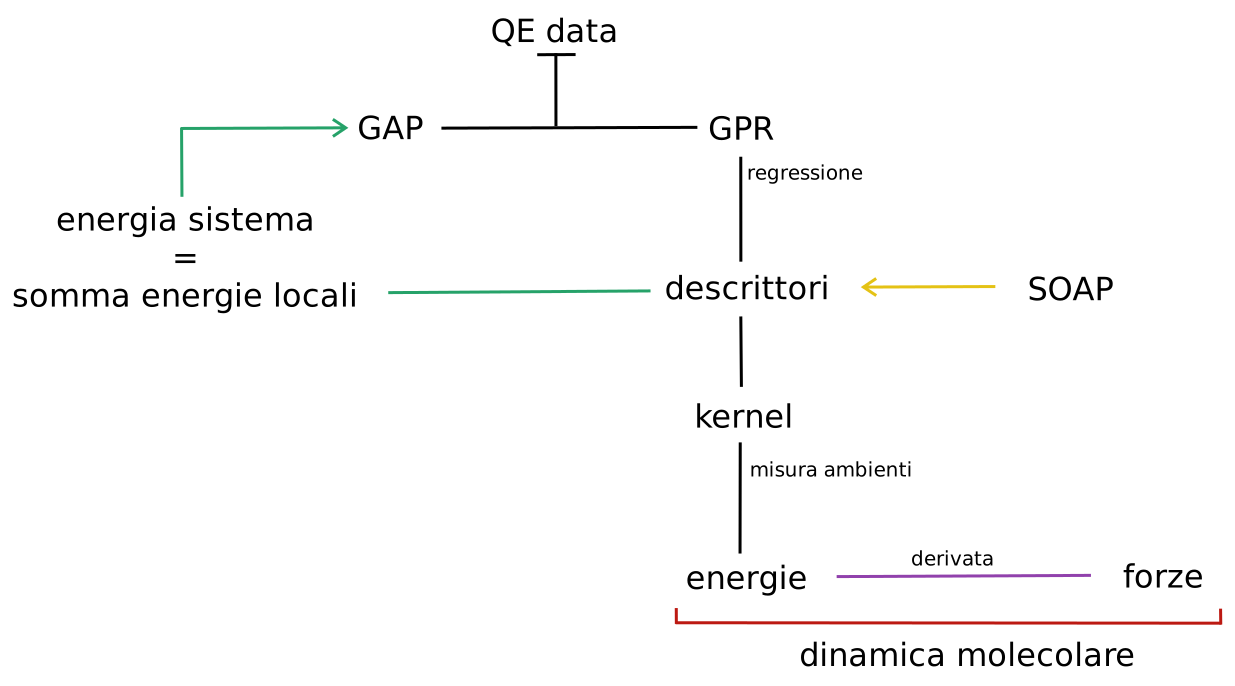
\includegraphics[scale=0.3]{./img/gap-schema.png}
    \captionof{schema}{Struttura schematica del framework GAP}
    \label{sch:schema-gap}
\end{figure}

Lo schema \ref{sch:schema-gap} descrive l'insieme di elementi che costituiscono il framework di un potenziale GAP.

Il processo matematico su cui si basa un potenziale GAP è la GPR (Gaussian Proces Regression). 
Essendo questo un argomento vasto, anche per le innumerevoli applicazioni, nel seguito diamo una breve spiegazione del suo funzionamento senza soffermarci su particolari dettagli.

Il GPR è un metodo di regressione non parametrico, questo significa che non assumiamo che la relazione tra i dati abbia una specifica forma funzionale.
Questo ci permette di modellizzare sia relazioni non note che relazioni complesse.

Il processo ci permette di utilizzare la coppia di dati $(x, f(x))$ per generare una previsione del valore di $f$ in un punto che non appartiene al set di dati.

Per fare questa previsione utilizziamo un kernel (indicato spesso con $K$), ovvero una funzione che ci permette di definire la somiglianza tra due punti di input, ad esempio $(x_1, x_2)$, questo ci permette di imporre che punti tra loro vicini diano risultati non dissimili.
Inoltre possiamo utilizzare i paraemtri del kernel per definire le interazioni tra i punti, infatti in base alla distribuzione dei dati potrebbe essere necessario far parlare tra loro punti lontati, come nel caso di periodicità, oppure limitare l'interazione solo ai prossimi vicini.


Volendo dare alcuni dettagli aggiuntivi, quello che andiamo a fare è considerare l'insieme di tutte le funzioni $f$ che passando per l'insieme di punti $D$, questo rappresenta i dati osservati.
Si costruisce una distribuzione di probabilità associata a queste funzioni, questa è una distribuzione gaussiana multivariata.
La funzione che cerchiamo è il valore di aspettazione di questa distribuzione e il kernel svolge il ruolo di matrice di covarianza.

Usiamo una spiegazione geometrica, nel caso più semplice possibile, per descrivere l'idea del processo, assumiamo di avere i dati $(x, f(x))$, possiamo assumere che $x$ segua una distibuzione gaussina la cui media sia proprio il valore $f(x)$.

Possiamo vedere una rappresentazione della distribuzione gaussiana nella seguente \ref{fig:curva-gaussiana}:

\begin{figure}[!h]
    \centering
    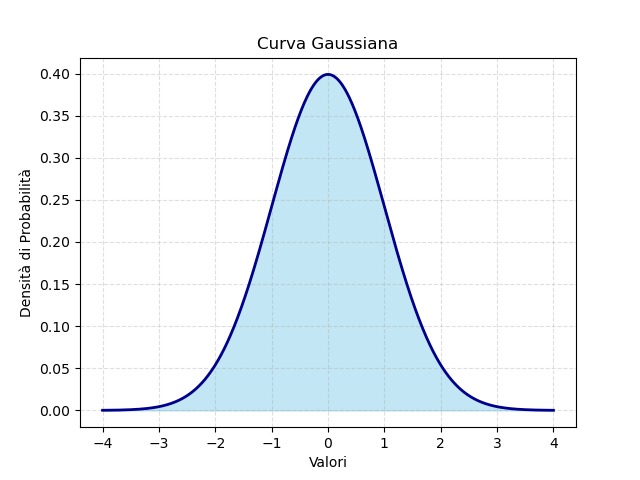
\includegraphics[scale=0.35]{./img/curva-gaussiana.png}
    \caption{Rappresentazione di una curva gaussiana}
    \label{fig:curva-gaussiana}
\end{figure}


Supponiamo adesso di voler prevedere il valore in un punto diverso che chiamiamo $x^*$. 
Consideriamo anche di aver precedentemente definito una funzione di kernel $K$, ricordiamo che questa dipende solo dai valori in input e non dai valori assunti dalla funzione.
Inoltre il valor medio di $f(x^*) = f^*$, lo conosciamo in quanto si assume un valore a priori, non entrando nei particolari, diciamo soltanto che si può assumere un valore sensato.
Abbiamo così costruito una distribuzione gaussiana bivariata.
Ricordando che sappiamo il valore di $f(x)$ possiamo "tagliare" la funzione bivariata in corrispondenza del noto $x$ e ottenere la distribuzione di $f^*$ dopo aver considerato i dati, da questa nuova distribuzione estraiamo il valor medio, esso è la nostra previsione.

La rappresentazione di questo concetto è data dalla seguente immagine \ref{fig:bi-gaussiana_e}:

\begin{figure}[!h]
    \centering
    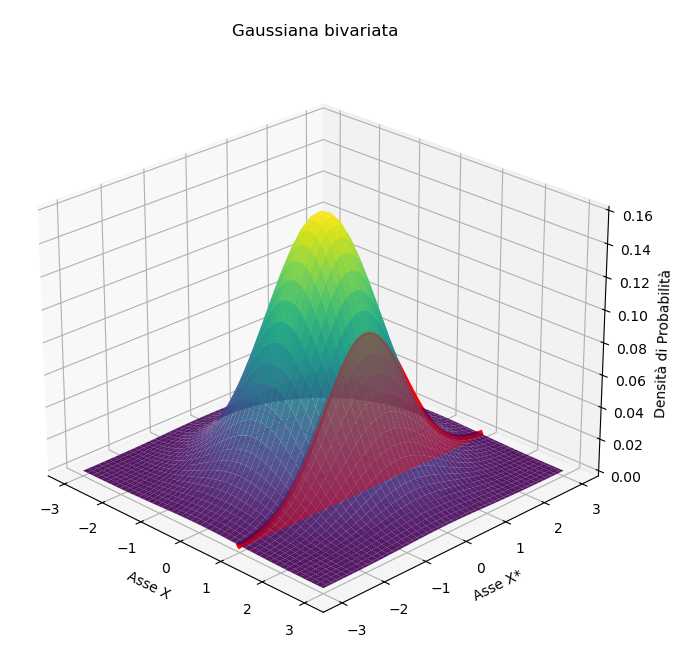
\includegraphics[scale=0.35]{./img/bi-gaussiana_e.png}
    \caption{Rappresentazione di una curva gaussiana bivariata, è evidenziato il taglio rispetto ad uno specifico valore di $x$}
    \label{fig:bi-gaussiana_e}
\end{figure}


Si generalizza, anche se con un pizzico di difficoltà, questo processo ad un numero arbitrario di valori di input.

Vogliamo notare come qui non abbiamo trattato la stima delle incertezze sulle previsioni e di come incorporare l'incertezza di misura (come noise) sui dati osservati.